%%%%%%%%%%%%%%%%%%%%%%%%%%%%%%%%%%%%%%%%%%%%%%%%%%%%%%%%%%%%%%%%%%%%%%
%     File: ExtendedAbstract_imple.tex                               %
%     Tex Master: ExtendedAbstract.tex                               %
%                                                                    %
%     Author: Andre Calado Marta                                     %
%     Last modified : 27 Dez 2011                                    %
%%%%%%%%%%%%%%%%%%%%%%%%%%%%%%%%%%%%%%%%%%%%%%%%%%%%%%%%%%%%%%%%%%%%%%
% A Calculation section represents a practical development
% from a theoretical basis.
%%%%%%%%%%%%%%%%%%%%%%%%%%%%%%%%%%%%%%%%%%%%%%%%%%%%%%%%%%%%%%%%%%%%%%

\section{System Description}

The short term objective of this work is to provide a solution for IST's immediate need of being able to know what assets it currently owns. In order to do so, we require some minimum information such as the asset's identification/title, location and the collection it belongs to.

In the medium to long term, the objective of this work is to provide an easily scalable asset management platform where developers are capable of, without much effort or prior knowledge, adding new information specific to new groups of assets as well as adding other new features to the system. Another long term objective is to then integrate the platform with other applications besides the FenixEdu system.

The proposed platform will follow a web architecture as shown in figure \ref{webArchitecture}.

\begin{figure}[h!]
    \centering
    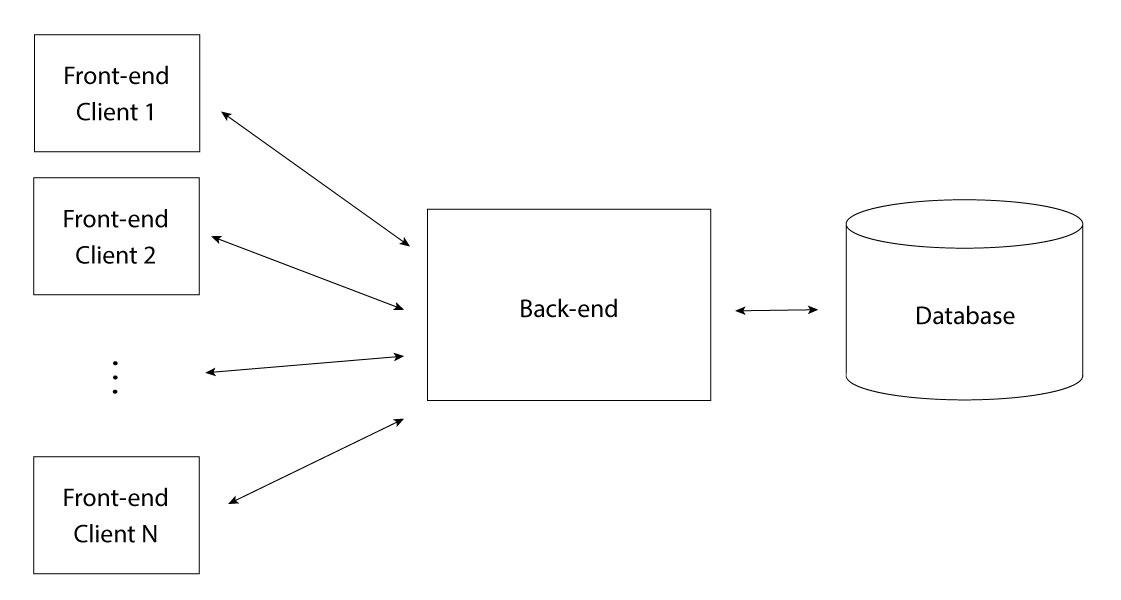
\includegraphics[scale=0.19]{images/Architecture/thesisArquitecture.jpg}
    \caption[Web architecture]{Commonly used web architecture that will serve as template for the platform.}
    \label{webArchitecture}
\end{figure}

%%%%%%%%%%%%%%%%%%%%%%%% DATA MODEL %%%%%%%%%%%%%%%%%%%%%%%%
\vspace{4mm}
\textbf{Data Model}
\vspace{2mm}

The main focus of this system is the way in which we will model our data. The most intuitive way of doing it would be having, for each asset, a node of information with all possible properties that the asset can have and only fill in the relevant properties for that specific asset. This would simplify our data structure since we would have the same structure for every single asset and would not have to create different structures for different assets. The problem here is that we would end up with vast amounts of irrelevant data fields as well as many properties without an associated value. 

A possible way of tackling this problem would be of creating a solution like the one presented in figure \ref{dataStructure1}.

\begin{figure}[h!]
    \centering
    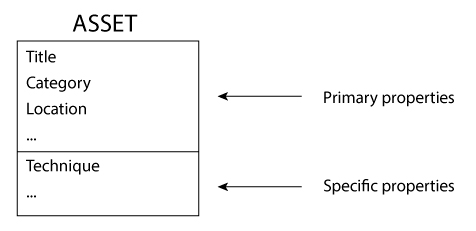
\includegraphics[scale=0.35]{images/Architecture/Data-structure-1.jpg}
    \caption[Data structure 1]{Initial data structure}
    \label{dataStructure1}
\end{figure}

In this data structure, we would define a couple of primary properties that would appear in all assets as well as a couple properties specific to the current asset. The specific properties would be conditional of the primary ones. This way, certain specific properties would be associated main properties' values. For example: an asset with the category of painting would only have, besides the primary properties associated to every assets, properties associated to paintings.

In this solution, an asset would have different sections (primary and specific ones) that are independent of each other. When relating this with the Spectrum standard \cite{CollectionsTrust2009TheProcedure} described in the previous chapter, we can divide each asset into multiple procedures where each procedure contains its properties. By doing this we are following the Spectrum standard as well and making the information associated to each procedure independent from each other.

\begin{figure}[h!]
    \centering
    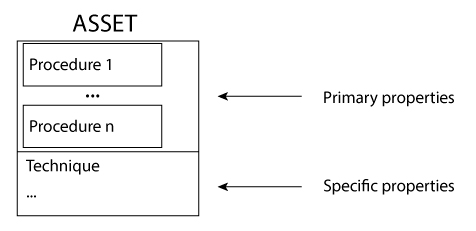
\includegraphics[scale=0.35]{images/Architecture/Data-structure-2.jpg}
    \caption[Data structure 2]{Spectrum procedure oriented data structure}
    \label{dataStructure2}
\end{figure}

Due to the limited timespan of this work, only a few key properties will be implemented. The chosen properties will be associated to the following groups and will provide IST with the minimum necessary information for cataloguing it's current asset collection:

\begin{itemize}
    \item Asset Identification
    \item Collection
    \item Asset Description
    \item Asset Location
    \item Asset History
\end{itemize}

Each one of these groups will include the minimum necessary information to identify an asset. These groups can be easily expanded to include more features as described in the full document of this work.

A possible solution for implementing the previously described data structure is JSON. JSON is a data format that allows for nesting variables, objects and arrays within each other, creating a simple to implement and read structure such as the tree associated to the specific properties. Another advantage of using JSON is the incorporation of this data format to other languages such as Javascript where a JSON element directly maps to a Javascript object \cite{Rischpater2015JavaScriptCookbook}.
    In listing \ref{assetJSON} an example of a possible asset JSON data structure is shown.
    
    \begin{lstlisting}[caption={Example of an asset's JSON data structure stored in the database.},label={assetJSON}]
{
    "_id" : 
    ObjectId("5d4d734bd1fa0"),
    "ObjectIdentification" : {
        "title" : 
        "Quadro da nascente",
        "optionalIds" : [
            {
                "N de inventorio B" : 
                "435"
            }
        ]
    },
    "ObjectDescription" : {
        "category" : [
            "Pinturas",
            "Gravuras"
        ]
    },
    "pinturas" : {
        "author" : "Eduardo Lopes",
        "year" : "2007",
        "material" : [
            "Madeira"
        ],
        "suporte" : "Madeira",
        "tecnica" : "Aguarela"
    },
    "gravuras" : {
        "amountOfCopies" : "252",
        "copyNumber" : "8"
    }
}
\end{lstlisting}

Specific modules can be associated to an asset depending on its category. In the previous listed example, we can observe that the data structure contains 2 objects which are conditionally inserted to the asset upon insertion: "pinturas" and "gravuras". The properties exist in the data structure since in the "ObjectDescription" both these properties are included. In this specific case "gravuras" is a sub-category of "pinturas", meaning that for an asset to have the property "gravuras" it must also have the property "pinturas".

%%%%%%%%%%%%%%%%%%%%%%%% DATA PERSISTENCE %%%%%%%%%%%%%%%%%%%%%%%%
\vspace{4mm}
\textbf{Data Persistence}
\vspace{2mm}

Now that the data structure is defined, we must ensure its persistance. This means that our data will survive even after the process that created it ends or if the system shuts down, to do so, a database is needed.

When thinking of a database choice in computer engineering the most popular option is using an SQL based system such as MySQL. A MySQL database is made up of multiple tables, with each table having a specific pre-defined data structure schema. In our museum example this means that we could have, for example, a table which contained all information of assets that were painting such as the author, technique, and so on. Each table then has rows, being that each row corresponds to a single item such as an asset. 

When looking into other database systems, another solution is using a document based database system such as MongoDB. In MongoDB, documents are grouped into collections, meaning that the database might have a collection for the assets, one for the users, and so on. When relating to MySQL, we can look at collections as being SQL tables and documents as being table rows. Documents follow a dynamic JSON structure, in this structure we can nest properties inside other properties \cite{MongoDB2016MongoDBGuide}. When comparing to the previously described SQL structure, in MongoDB collections do not have an associated data schema, meaning that they may contain assets with different properties. This solves the previously presented problems of using an SQL based system for managing museum assets.

In addition to this, the data model introduced in the previous section can be easily implemented by subdividing the content of each asset's documents into multiple independent modules.

%%%%%%%%%%%%%%%%%%%%%%%% BACK-END %%%%%%%%%%%%%%%%%%%%%%%%
\vspace{4mm}
\textbf{Back-end}
\vspace{2mm}

Having defined the data structure as well as the database the next step is to define how the necessary computing power will be implemented in order to perform operations on the database. Having users directly interacting with the database may bring problems such as data duplication or insertion of invalid data structures, which will compromise the whole system.

In order to prevent such problems a back-end infrastructure is defined. In this case, the back-end infrastructure will consist of the previously mentioned MongoDB database as well as a machine running processes capable of performing the standard database operations as well as ensuring the system's integrity.

An example such solution is using Node.js: an open-source, cross-platform JavaScript run-time environment that executes Javascript code outside of a browser in order to enable server-side scripting \cite{Corporation2019Node.jsGuide}. Since JSON and MongoDB documents perfectly map into Javascript objects, performing the necessary data conversions will be a seamless process. Throughout the rest of the work, this Node.js environment will be refered to as the back-end.

The back-end is based on routes which are identified by a unique URL according to the REST methodology \cite{GregorioIntroREST}. This means that in order for a user to interact with the system a request is sent, according to the REST API to the corresponding back-end route. So for example, in order to get the list of users in the database we will perform an HTTP GET request to a route similar to this one:

\textbf{GET}
\textbf{http://www.myServer.com/api/users}

Our back-end server will receive this request, access the database, insert all of the users into a javascript array and send that array to the front-end.

\begin{figure}[h!]
    \centering
    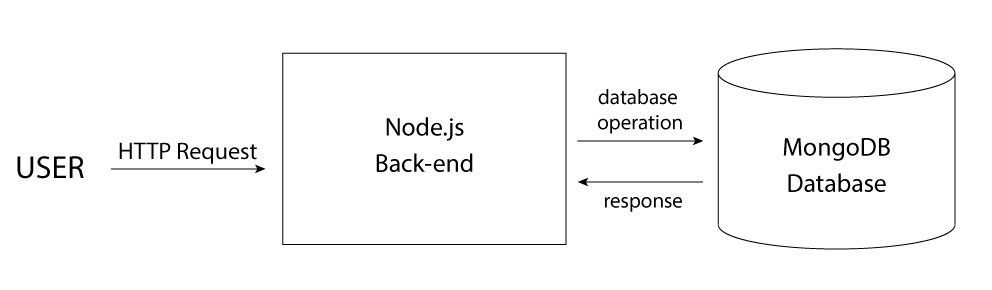
\includegraphics[scale=0.23]{images/Backend/backendRequest.jpg}
    \caption[Back-end request]{User performing a request to the back-end.}
    \label{backendRequest}
\end{figure}

This is a very basic example which does not include authentication. Security and user authentication will be discussed further on.

%%%%%%%%%%%%%%%%%%%%%%%% FRONT-END %%%%%%%%%%%%%%%%%%%%%%%%
\vspace{4mm}
\textbf{Front-end}
\vspace{2mm}

Performing an HTTP request to a web server requires some computer networking knowledge, leaving the system as it is now would only allow a reduced number of people to use it. It is possible to abstract all of the networking logic into something such as a browser interface with interactive buttons and data visualizations. This is called the front-end.

The front-end corresponds to the user interface with which the user will interact without the need of knowing any prior knowledge about programming. This is a case of code on demand, in order for the user to be able to use the platform we will simply need to open a web browser and type in the URL corresponding to the server directory in which the front-end files are stored. By doing this, the browser will send the necessary HTTP request to the server in order to get the interface code and will display it on the browser for the user to interact with.

In order to implement the front-end a framework called Vue.js (or simply Vue) can be used. Vue is a web development framework created by Evan You in 2013 after having worked for Google using the framework Angular.js in various projects. This framework allows us to separate the various parts of the platform into components. A component is a file which can contain HTML, CSS and Javascript code. We use components in order to better structure our code, it would be a mess if we had all the elements of our platform into the same HTML, CSS and Javascript files. Having the possibility of dividing the platform into components will prove to be very important in order to create a scalable code base where each element works independently from each other \cite{Copes2018VueHandbook}.

The code structure used for our front-end client is quite similar to the one seen in most Vue projects, the big difference is the way in which we use modules to create a truly dynamic and scalable platform. We define views that serve as the containers for other components but you can also look at views as if they correspond to each of our platform's different pages.

The big challenge with storing museological assets lies in their massive diversity of properties. It makes sense to specify what type of motor a car has but it does not make sense to specify what type of a motor a painting has. This is where our modules come in.

The main operations of the platform are the following:

\begin{itemize}
    \item Insert - Add a new asset to the database.
    \item Display - Observe an asset's details.
    \item Edit - Change an asset's details.
    \item Search - Search for assets with certain caracteristics.
    \item Config - Configure the values that a user can select for a specific module.
\end{itemize}

By defining these key operations we can now separate our assets' components into different modules. We have, for example, the object identification module which includes an asset's title and optional ids. For this module we will have insert, display, edit, search and config files.

\begin{figure*}[h!]
    \centering
    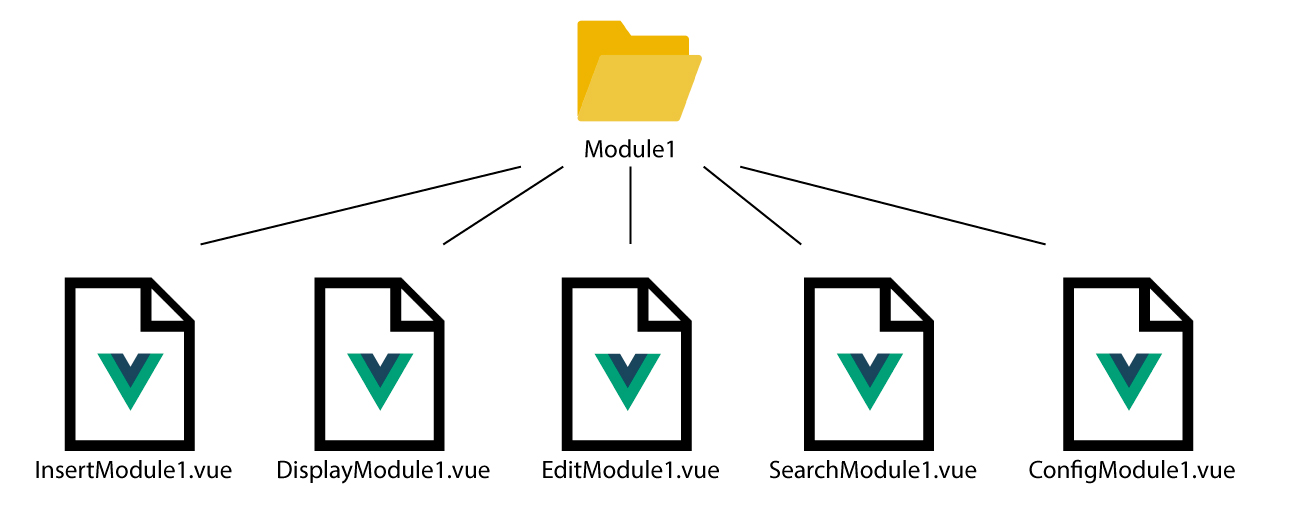
\includegraphics[scale=0.3]{images/Frontend/moduleStructure.jpg}
    \caption[Front-end module structure]{Module structure in front-end.}
    \label{moduleStructure}
\end{figure*}

This means that when displaying an asset we will render in our web page all of the modules relevant to the asset, thus creating a single information page that results from many Vue components. We can now also decide which modules we show to the user depending for each case. When displaying an asset we will view its categories and render all of modules corresponding to those categories if they exist, this is done dynamically in Vue by conditionally rendering Vue components.

In order to further illustrate the relation between a module and other components we can observe figure \ref{frontendStructure}.

\begin{figure}[h!]
    \centering
    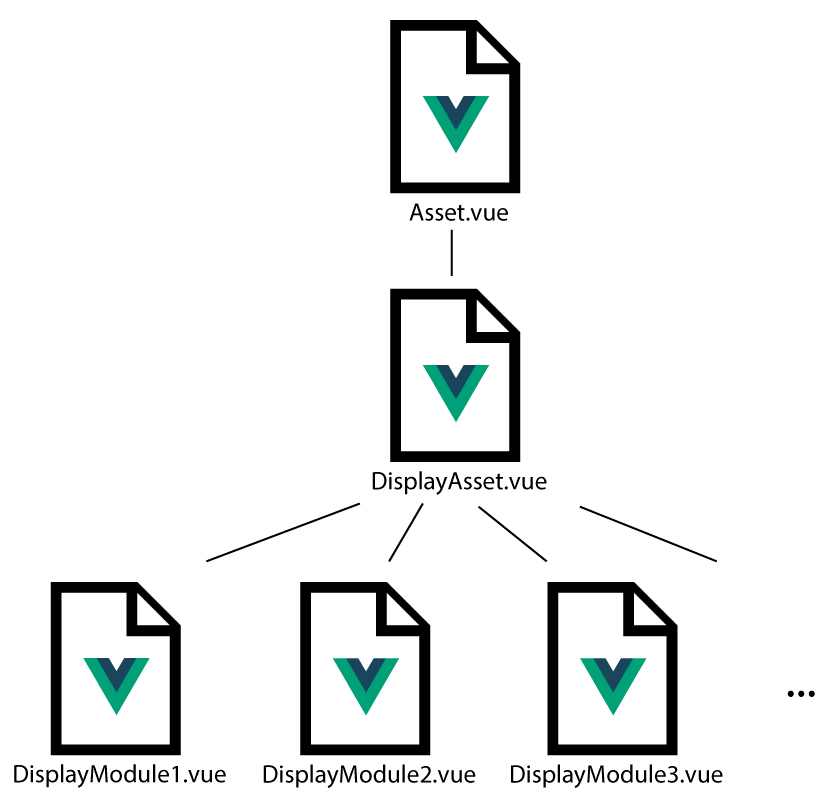
\includegraphics[scale=0.23]{images/Frontend/frontendStructure.jpg}
    \caption[Front-end file structure]{Example of how display modules are connected to parent components.}
    \label{frontendStructure}
\end{figure}

The front-end is tightly coupled to the back-end, meaning that it won't function properly without a running back-end server. Data that we view on the interface, such as the name of the assets, has to be fetched from the database. In order to get such data we perform HTTP requests to the back-end server. But using simple HTTP request is not enough since we want to load the data on the page dynamically and not have to refresh the page each time we make a request. For that we use AJAX in order to perform asynchronous requests to the server. An asynchronous operation allows us to perform other tasks while waiting for this operation to complete \cite{Gyorodi2016WebAjax}. After fetching the data, we can then process it and display it in our Vue component. Our system architecture will now resemble the one in figure \ref{exampleGET}.

\begin{figure}[h!]
    \centering
    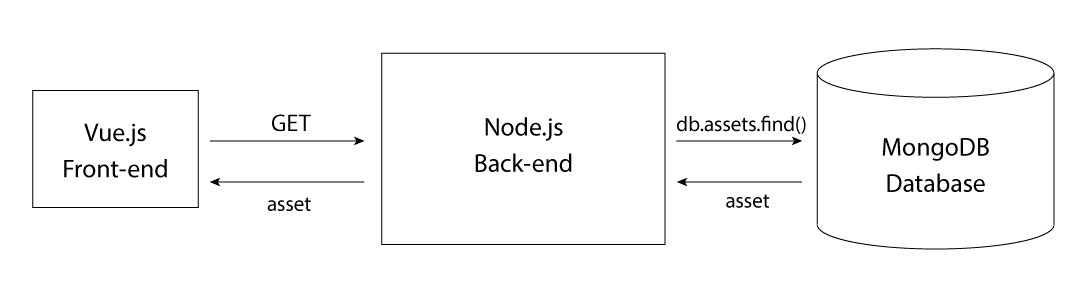
\includegraphics[scale=0.21]{images/Frontend/getAssetExample.jpg}
    \caption[Front-end request example]{Example of a client request for an asset.}
    \label{exampleGET}
\end{figure}

%%%%%%%%%%%%%%%%%%%%%%%% SECURITY AND AUTHENTICATION %%%%%%%%%%%%%%%%%%%%%%%%
\vspace{4mm}
\textbf{Security and Authentication}
\vspace{2mm}

Security is of key importance to our web platform since we have multiple users acessing common data on the database. We need to have a way of defining specific permissions for each user in order to control what they can and cannot do. We start by defining 3 types of possible user profiles:

\begin{itemize}
    \item Viewers - Can only view the assets in the database, they cannot change or delete anything.
    \item Editors - Can insert, edit and delete assets from the categories they have been assigned.
    \item Admins - Can do everything. This includes giving permissions to other users, configuring modules' data and inserting, editing and deleting any assets from the database.
\end{itemize}

To implement this security system we use JWT as well as the FenixEdu authentication system \cite{Silva2002TheProject} since we only want to allow users from IST to use our application for now.


JWT is used for passing tokens between machines in order to identify and validate who is sending the request \cite{Shingala2019JSONMQTT}. In our platform, the front-end will append a token to requests that require one. For example, editing is a higher permission feature which viewers must be unable to use. To make sure the person editing the asset can indeed do it we append a token that confirms the person's identity. Most requests such as a search query do not require the front-end to append a token to the message since every type of user can perform this action. Once the back-end receives a request, it will decode the token in order to identify the person performing the action. For this, it will need to know the secret with which the token was encrypted with, but that is no problem since the only entity that generates tokens is the back-end itself.

This is the authentication process:

\begin{enumerate}
    \item The front-end redirects the user to the FenixEdu login page.
    \item If the login is successfull, FenixEdu will redirect the user back to the front-end and append a code to the URL.
    \item The front-end sends a POST request to FenixEdu with the received code.
    \item FenixEdu responds with a token corresponding to the user's session.
    \item The front-end sends that token to the back-end
    \item The back-end gets the user's basic information from FenixEdu.
    \item The back-end checks if the user is already in the database, if not, a new user is created. The user university id is used as the user identifier.
    \item The back-end generates a jwt token and sends it as a response to the front-end.
    \item The front-end stores the jwt token locally and appends it to future requests when needed.
    \item Each time the back-end receives a jwt token, it decodes it and views if the user has the required permissions before continuing.
\end{enumerate}

The front-end checks, each time before we change pages, if the token is already in the front-end, if it is, the user will continue to the desired page. If not, the authentication process that can be seen in figure \ref{securityFlow} will be triggered in order to authenticate the current user.


\begin{figure}[h!]
    \centering
    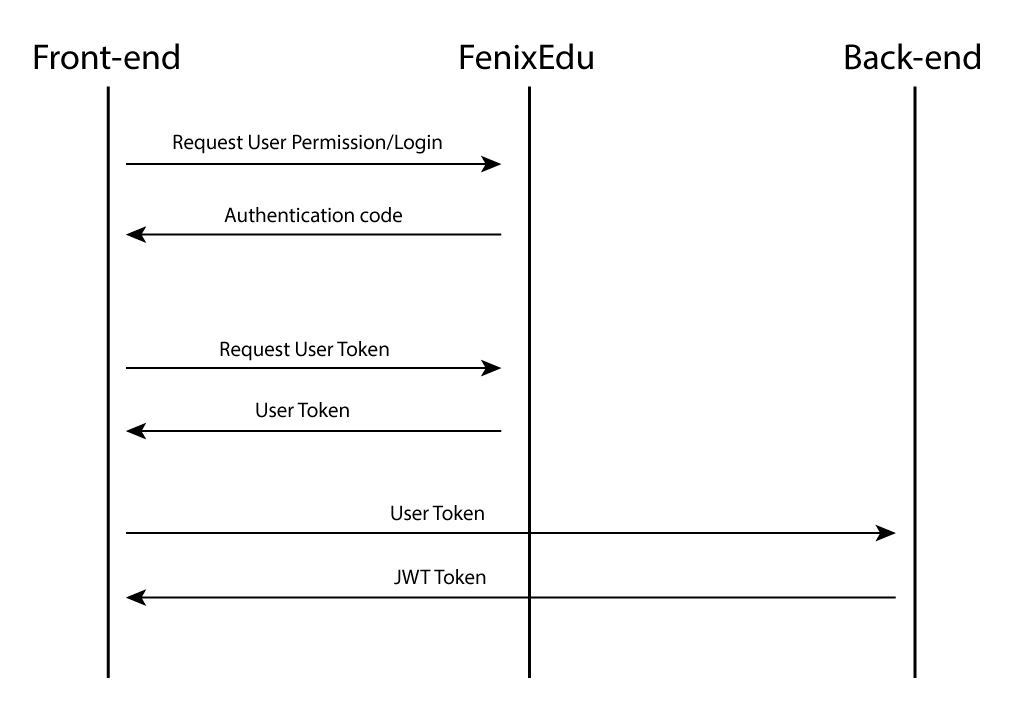
\includegraphics[scale=0.24]{images/Security/securityFlow.jpg}
    \caption[Login process]{User authentication process.}
    \label{securityFlow}
\end{figure}

%%%%%%%%%%%%%%%%%%%%%%%% CATEGORY MATCHING %%%%%%%%%%%%%%%%%%%%%%%%
\vspace{4mm}
\textbf{Category Matching}
\vspace{2mm}

In order to implement the dynamic modules previously described we require a way of identifying the categories of the asset. This information is included in the asset's JSON, more specifically in the Object Description object. In this object is included the information that associates the asset to certain categories in order to then allow for other dynamic modules to work. These categories follow a tree structure. This allows for the user to specify, within a category, the asset's sub categories in order to further identify the asset.
An example of a category tree is shown in figure \ref{paintingsTree}. In this example we can set an asset's category as being a painting and then drill down even further and state, for example, that it is also of the category acrylic.

\begin{figure}[h!]
    \centering
    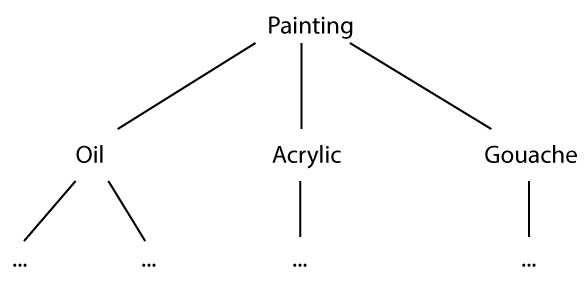
\includegraphics[scale=0.4]{images/Architecture/paintingsTree.jpg}
    \caption[Category tree example]{Example data structure of a category.}
    \label{paintingsTree}
\end{figure}

%%%%%%%%%%%%%%%%%%%%%%%% WEB PLATFORM %%%%%%%%%%%%%%%%%%%%%%%%
\vspace{4mm}
\textbf{Web Platform}
\vspace{2mm}

The work developed is based on a web architecture. This implies communication between machines, more concretely between: the front-end, back-end and database. Another option for this platform would be using other technologies to develop a solution with all of these 3 elements working locally in the same machine. Having a local solution would have its benefits when it comes to, for example, security since we would know exactly who could access the platform. The major drawback would be that the platform could only be accessed from a specific machine and only the people with access to that machine would be able to interact with our platform.


Right from the beginning it was known that this platform would have to be extremely convenient to use in order for museum collectors to make use of it. That is why the platform is based on a web architecture. This allows for collectors to manage their collections from any device and any place as long as they have an internet connection. Another advantage of having a web platform is that we can give the collectors the option of allowing the general public to view their collections without the ability to perform the same actions as the collection managers. But having these benefits comes with a price, and that is the need for more complex security systems in order to avoid that people who do not have permissions to edit the collections do so.


Another advantage of using a web platforms with these specific technologies is the ease of developing new features since javascript is currently one of the most popular programming languages amongst developers as well as being a higher-level programming language when comparing to others such as C or C++ in which the developers have to deal with concepts such as memory allocation and pointers which are abstracted in javascript.


When it comes to the choice of technologies for developing our web platform solution another choice of programming language would be using Python with, for example, the framework Django for the front-end and the framework Flask for the back-end \cite{Langtangen2015UsingApplications}. This would wield a very similar result, despite this observation, javascript was chosen for its popularity when it comes to web development since anyone with minimum knowledge of javascript would be able to quickly learn and implement small features in the current platform.